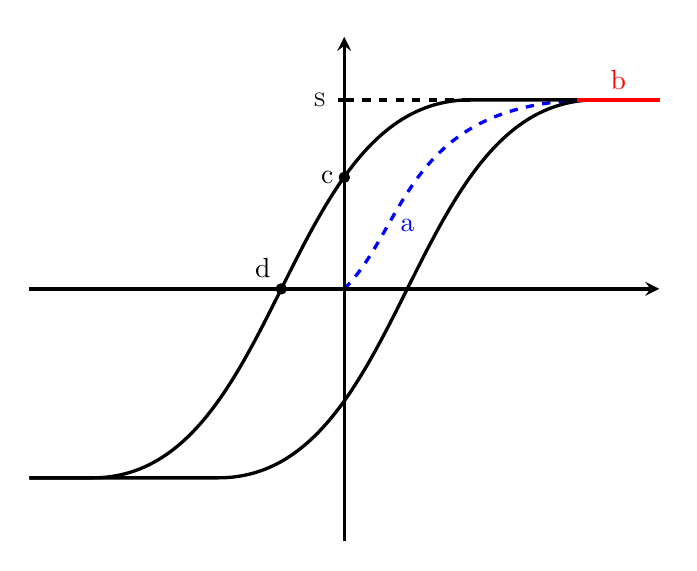
\begin{tikzpicture}[line width = 1.2pt, line join=round,x=1cm,y=1cm,>=stealth, scale = 0.8]
	% Neukurve
	\draw [dashed, color=blue] (0,0) to [controls={+(1,1) and +(-3,0)}] (4,3) -- (5,3);
	% Koordinatensystem
	\draw [->] (-5,0) -- (5,0) node [anchor = north] {$ \HFeld $};
	\draw [->] (0,-4) -- (0,4) node [anchor = east] {$ \Magnetisierung $};
	% Sättigungs Magnetisierung
	\draw [dashed] (2,3) -- (0,3);
	\draw (0.1,3) -- (-0.1,3) node[anchor=east] {$ \Magnetisierung_\mathrm{S} $};
	% Hysteresekurve
	\draw (-5,-3) -- (-4,-3) to [controls={+(3,0) and +(-3,0)}] (2,3) -- (5,3);
	\draw (5,3) -- (4,3) to [controls={+(-3,0) and +(3,0)}] (-2,-3) -- (-5,-3);
	% Erläuterungen
	\draw [color=blue] (1,1) node {a};
	\draw [color=red] (3.7,3) -- (5,3) node [anchor=south,midway] {b};
	\filldraw (0,1.77) circle (1.8pt) node [anchor = east] {c};
	\filldraw (-1,0) circle (1.8pt) node [anchor=south east] {d};
\end{tikzpicture}